%%%%%%%%%%%%%%%%%%%%%%%%%%%%%%%%%%%%%%%%%%%%%%%%%%%%%%%%%%%%%%%%%%%%%%%%
%                                                                      %
%     File: Implementation/04_ManeuversAndMissions.tex                 %
%     Tex Master: ../Thesis.tex                                        %
%                                                                      %
%%%%%%%%%%%%%%%%%%%%%%%%%%%%%%%%%%%%%%%%%%%%%%%%%%%%%%%%%%%%%%%%%%%%%%%%

% ==============================================================================
\section{Manoeuvres and Missions}
\label{sec:maneuvers_and_missions}

% What produces the references that the controllers follow?
The controllers of Section~\ref{sec:controller_implementation} follow the references they are given, but do not decide where each vehicle should go. This is the role of the manoeuvres, which turn a simple motion, such as an orbit around the \gls{usv} or a landing on its deck, into the reference of each controller at every instant. The missions then chain these manoeuvres, for both vehicles, into a complete operation.

\subsection{Manoeuvres}
\label{subsec:maneuver_primitives}

% What is a manoeuvre?
A manoeuvre gives the reference of one vehicle as a function of time, sampled over the horizon of the controller at every instant. Five manoeuvres were defined for the \gls{uav}, takeoff, formation, orbit, chase and landing, and four for the \gls{usv}, which holds its position, follows a route of waypoints, pursues a target, keeping a safe distance from it, or supports the \gls{uav}. Each is set by a few parameters, such as a destination or a speed. The references are simple geometric curves in time, such as lines and circles, since the controllers keep the vehicles within their limits whatever reference they are given, even a single point.

% Relative to what are the references given?
Most manoeuvres of the \gls{uav} are given relative to the winch, since the vehicle works around the \gls{usv} and must return to it. Their references move with the \gls{usv} along the trajectory predicted by its controller, either in fixed axes or in the axes of the \gls{usv}, so that they turn with it, as when the \gls{uav} scouts ahead of the bow. The height is taken above the mean height of the winch, so that the \gls{uav} does not follow the heave of the deck. The point of the formation and the centre of the orbit can also be fixed in the world, to reach or circle a structure, and the chase follows the target.

% How does the USV support the UAV?
When the \gls{uav} works around a structure, the tether may not reach far enough for it to go all the way around. The \gls{usv} then supports it, taking as its reference the point on the water below the reference of the \gls{uav}, pushed away from the structure to a safe distance, so that it follows the \gls{uav} and gives it the reach of the tether. This is only possible when the reference of the \gls{uav} is fixed in the world, since a reference given relative to the winch would move with the \gls{usv}, and each vehicle would then chase the other.

% Where does the UAV look?
Each manoeuvre also sets the heading of the \gls{uav}, through a point that the vehicle looks at, or away from, such as the winch, a structure or a target, so that a camera on the vehicle keeps it in view. For the takeoff and the landing it follows instead the heading of the \gls{usv}, which aligns the vehicle with the deck.

% What do the manoeuvres look like in practice?
Figure~\ref{fig:maneuver_catalogue} shows the manoeuvres of the \gls{uav} as performed in the missions of Section~\ref{subsec:missions_coordination}, seen from above in fixed axes, with the two vehicles drawn at the same instants, the older ones more transparent, so that their motion can be seen together. The formation (b) keeps the \gls{uav} ahead of the bow, in the axes of the \gls{usv}, while it follows a route, and the orbit (c) circles the \gls{usv} as it sails, shown in its axes, where the orbit is a circle, while in (d) the \gls{uav} orbits the \gls{usv} on patrol until it detects a target, which it then chases (e) as the \gls{usv} pursues it. The takeoff and the landing (a, f) are shown instead through the height of the \gls{uav} above the mean height of the winch, which shows the heave of the deck.

\begin{figure}[htbp]
    \centering
    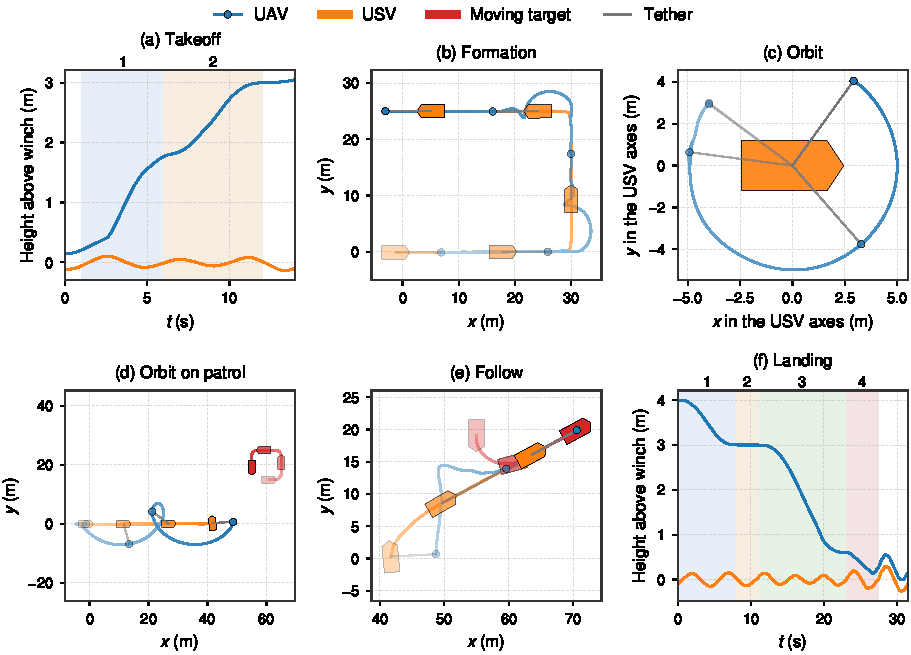
\includegraphics[width=\textwidth]{Implementation/figures/04_maneuvers_and_missions/maneuver_catalogue.pdf}
    \caption{Manoeuvres performed in simulation.}
    \label{fig:maneuver_catalogue}
\end{figure}

% How does the UAV take off from the moving deck?
The takeoff and the landing are the manoeuvres in which the \gls{uav} is closest to the deck and moves with it. To hold the vehicle against the deck, so that the waves do not tip it over and throw it into the sea, the winch can pull the tether with a constant force, which it applies at the start of the takeoff and keeps until the \gls{uav} is clear of the deck. The takeoff therefore begins with a vertical climb off the pad, phase~1 in Figure~\ref{fig:maneuver_catalogue}a, and only then moves the vehicle to its first position, phase~2, so that it does not drift over the edge of the deck at low height.

% How does the UAV land on the moving deck?
The landing is divided into four phases, shown in Figure~\ref{fig:maneuver_catalogue}f. The \gls{uav} first moves above the winch (1) and waits until it is centred above the pad and moving with it (2). It then descends with the winch pulling it towards the deck (3), and ends with a slow final approach towards a point below the deck (4), so that it touches down even if the deck falls away, and the speed of the contact is set by the heave rather than by the descent. Once it rests on the pad, the vehicle is disarmed, and the winch keeps it against the deck.

\subsection{Missions}
\label{subsec:missions_coordination}

% What is a mission?
A mission is a file with two sequences of manoeuvres, one for each vehicle. Each manoeuvre ends when a condition is met, either an event, such as the detection of a target, or the end of a manoeuvre of the other vehicle.

% What happens when something goes wrong?
A mission is aborted when a manoeuvre fails, when it takes too long, or when the operator requests it. The \gls{usv} then holds its position and the \gls{uav} lands.

% Which missions were tested?
Three missions were tested in simulation, shown in Figure~\ref{fig:missions}. In the scout (a), the \gls{uav} flies ahead of the bow. In the inspection (b), it circles a tower while the \gls{usv} supports it. In the patrol (c), it orbits the \gls{usv} until it detects a target, which it then chases while the \gls{usv} pursues it.

\begin{figure}[htbp]
    \centering
    \tikzset{
        mbox/.style={draw, rounded corners=2pt, minimum height=0.6cm, inner sep=3pt, font=\footnotesize},
        mlink/.style={-{Stealth}, semithick},
        mcond/.style={font=\scriptsize, text width=1.5cm, align=center, inner sep=2pt},
        mend/.style={circle, fill, inner sep=0pt, minimum size=5pt},
        vlabel/.style={anchor=east, font=\footnotesize\bfseries}}
    \subfloat[Scout.]{
    \begin{tikzpicture}
        \node[vlabel] at (0, 0) {\gls{uav}};
        \node[mbox, anchor=west] (uav0) at (0.2, 0) {Takeoff};
        \node[mbox, right=1.55cm of uav0] (uav1) {Formation};
        \draw[mlink] (uav0) -- node[mcond, above] {in position} (uav1);
        \node[mbox, right=1.55cm of uav1] (uav2) {Landing};
        \draw[mlink] (uav1) -- node[mcond, above] {route ended} (uav2);
        \node[mend, right=1.55cm of uav2] (uavend) {};
        \draw[mlink] (uav2) -- node[mcond, above] {touchdown} (uavend);
        \node[vlabel] at (0, -1.0) {\gls{usv}};
        \node[mbox, anchor=west] (usv0) at (0.2, -1.0) {Hold};
        \node[mbox, right=1.55cm of usv0] (usv1) {Route};
        \draw[mlink] (usv0) -- node[mcond, below] {\gls{uav} ahead of the bow} (usv1);
        \node[mbox, right=1.55cm of usv1] (usv2) {Hold};
        \draw[mlink] (usv1) -- node[mcond, below] {last waypoint} (usv2);
    \end{tikzpicture}}
    \\[2mm]
    \subfloat[Inspection.]{
    \begin{tikzpicture}
        \node[vlabel] at (0, 0) {\gls{uav}};
        \node[mbox, anchor=west] (uav0) at (0.2, 0) {Takeoff};
        \node[mbox, right=1.55cm of uav0] (uav1) {Formation};
        \draw[mlink] (uav0) -- node[mcond, above] {in position} (uav1);
        \node[mbox, right=1.55cm of uav1] (uav2) {Orbit};
        \draw[mlink] (uav1) -- node[mcond, above] {\gls{usv} at the tower} (uav2);
        \node[mbox, right=1.55cm of uav2] (uav3) {Landing};
        \draw[mlink] (uav2) -- node[mcond, above] {lap covered} (uav3);
        \node[mend, right=1.55cm of uav3] (uavend) {};
        \draw[mlink] (uav3) -- node[mcond, above] {touchdown} (uavend);
        \node[vlabel] at (0, -1.0) {\gls{usv}};
        \node[mbox, anchor=west] (usv0) at (0.2, -1.0) {Hold};
        \node[mbox, right=1.55cm of usv0] (usv1) {Route};
        \draw[mlink] (usv0) -- node[mcond, below] {\gls{uav} took off} (usv1);
        \node[mbox, right=1.55cm of usv1] (usv2) {Support};
        \draw[mlink] (usv1) -- node[mcond, below] {last waypoint} (usv2);
        \node[mbox, right=1.55cm of usv2] (usv3) {Hold};
        \draw[mlink] (usv2) -- node[mcond, below] {lap covered} (usv3);
    \end{tikzpicture}}
    \\[2mm]
    \subfloat[Patrol.]{
    \begin{tikzpicture}
        \node[vlabel] at (0, 0) {\gls{uav}};
        \node[mbox, anchor=west] (uav0) at (0.2, 0) {Takeoff};
        \node[mbox, right=1.55cm of uav0] (uav1) {Orbit};
        \draw[mlink] (uav0) -- node[mcond, above] {in position} (uav1);
        \node[mbox, right=1.55cm of uav1] (uav2) {Chase};
        \draw[mlink] (uav1) -- node[mcond, above] {target detected} (uav2);
        \node[mbox, right=1.55cm of uav2] (uav3) {Landing};
        \draw[mlink] (uav2) -- node[mcond, above] {target intercepted} (uav3);
        \node[mend, right=1.55cm of uav3] (uavend) {};
        \draw[mlink] (uav3) -- node[mcond, above] {touchdown} (uavend);
        \node[vlabel] at (0, -1.0) {\gls{usv}};
        \node[mbox, anchor=west] (usv0) at (0.2, -1.0) {Hold};
        \node[mbox, right=1.55cm of usv0] (usv1) {Route};
        \draw[mlink] (usv0) -- node[mcond, below] {\gls{uav} took off} (usv1);
        \node[mbox, right=1.55cm of usv1] (usv2) {Pursuit};
        \draw[mlink] (usv1) -- node[mcond, below] {target detected} (usv2);
        \node[mbox, right=1.55cm of usv2] (usv3) {Hold};
        \draw[mlink] (usv2) -- node[mcond, below] {target intercepted} (usv3);
    \end{tikzpicture}}
    \caption{Missions tested in simulation.}
    \label{fig:missions}
\end{figure}
